\documentclass{article}
    \usepackage[export]{adjustbox}
	\usepackage[english]{babel}%required allways
	\usepackage{booktabs, makecell}	%required for bookstyle tables, without these the tables will have to be redrawn
 \renewcommand\theadfont{\bfseries}
 \renewcommand{\cellalign}{cl}
	\usepackage{bm}
	\usepackage[T1]{fontenc}
\usepackage{lmodern}
\usepackage{chngcntr}
	\usepackage{tikz}		% required for linestyle graphics
 %   \usepackage{tikz,pgfplots}	
	\usepackage{enumerate}
	\usepackage{float} 		% required for example and excercise styles
   % \usepackage{chicago}
	\usepackage[round]{natbib}
    \usepackage{epstopdf}
    \usepackage[toc,page]{appendix} % required for adding appendice
	\usepackage[intlimits]{amsmath}%provide option intlimits to
    \usepackage{amsfonts}
							% give boundaries of limits above/below integral sign
	\usepackage{rotating} 	%required for rotated tables
	\usepackage{graphicx} 	%required for including external graphics files
\usepackage{ae,aecompl}
\usepackage{amsmath,amsthm,amssymb,enumerate,mathrsfs}
        \numberwithin{equation}{section}
    \usepackage{epsfig}
\usepackage[pdftex]{hyperref}
	\usepackage{caption}
    \usepackage{multirow}
    \usepackage{epsfig}    %required to put multiple figures under one caption
    \usepackage{lscape}    % change the layout of single page to landscape
    \usepackage{caption}
  %  \usepackage{subcaption}%required to add sub-captions
    \usepackage{subfig}
    \usepackage{setspace}
    \usepackage{url}
    \usepackage{multirow}
    \usepackage{multicol}
    \usepackage{bigstrut}
    \usepackage{natbib}
    \usepackage{bbm}
		\usepackage[a4paper]{geometry}
    \doublespacing
		\geometry{hscale=0.7,vscale=0.75,centering}
\def\R{{\rm I} \negthinspace {\rm R}}
\renewcommand{\baselinestretch}{1.50}\normalsize
\setlength\parindent{0pt}
\theoremstyle{plain}
\newtheorem{ro}{Corollary}
\newtheorem{prop}{Proposition}
\newtheorem{thm}{Theorem}

\theoremstyle{definition}
\newtheorem{de}{Definition}
\newtheorem{lm}{Lemma}
\newtheorem{exm}{Example}
\theoremstyle{remark}
\newtheorem{Alg}{Algorithm}
\newtheorem{rem}{Remark}
\bibliographystyle{agsm}
\hypersetup{
  colorlinks=true,
  linkcolor=blue,
  citecolor=blue,
  urlcolor=blue}
%\doublespace
\let\code=\texttt
\begin{document}

\begin{center}
%\maketitle
\setlength{\unitlength}{2cm}

{\Large Responses to Associate Editor and Referee's Comments \\[%
0pt]
\vspace{0.02in}
\large\textbf{Constructing hierarchical time series through clustering: \\Is there an optimal way for forecasting?}}
\end{center}


\noindent We greatly appreciate the time and effort the Associate Editor and the two referees have dedicated to reviewing our paper. The comments received are extremely insightful and have largely benefited the manuscript. We have revised the manuscript based on these comments and provided the following point-by-point response to the Associate Editor and two anonymous referees.
\vspace{-0.4in}
%\section*{\large Major points}
%We are glad that you find the topic important and interesting. 
%\medskip
%\medskip
\section*{Comments from the Associate Editor}
%\vspace{-0.1in}

\textit{The two reviewers find the paper well-written and a good fit for IJF - I agree. They provide some useful comments that will help the authors improve their manuscript, including the provision of additional consideration in the middle levels of the hierarchy in terms of hierarchy construction but also evaluation and a better description of the permutation algorithm. Overall, I think the comments can be fully addressed and I am looking forward to receiving a revised version of the paper.}

\medskip
\noindent \textbf{Authors' response:}
We express our gratitude to the Associate Editor for your guidance on the revision of this manuscript. In response to the suggestions and comments from the referees, we have conducted major and thorough revisions of the manuscript. Please see below a summary of the major changes we have made. %\\
\vspace{-0.03in}
\begin{itemize}
    \item We have enhanced the literature review by including more relevant studies in the discussion, thereby emphasizing the contribution of our research. This addresses Referee 1's comments. 
    \item We have conducted additional analyses on the performance of our methods on the intermediate levels defined by the natural hierarchies, where we used a bottom-up approach for clustering-based hierarchies. This addresses Referee 1's comments. 
    
    \item We have included a grouped hierarchy structure, which combines the aggregation constraints of all the clustering-based hierarchies. This addresses Referee 1's comments. 

    \item We have added a more detailed description of the permutation method in Section 4 of the manuscript. This addresses Referee 2's comments.

    \item We have included additional discussions in Section 3.3, on the competitive performance of the natural hierarchy in our studies. This addresses Referee 2's comments.

    \item {We have made our code and data available in a public GitHub repository to enable replication of the results presented in the manuscript. The repository can be accessed at: \url{https://github.com/Purity3-cyber/constructing_hierarchies}.}
    
\end{itemize}


In summary, the paper has greatly benefited from the insightful comments received. We hope that, the incorporation of these changes will now make the revised version suitable for \textit{International Journal of Forecasting}. 

\clearpage 
\newpage 


\section*{Comments from Referee 1}

% We appreciate your comments, and we are pleased that the referee acknowledged the significant challenges addressed in our research. Following the referee's guidance, we provide further clarifications and discussions which have made the paper more cohesive. We have also conducted additional analysis and comparisons, thereby emphasizing the contributions of the paper. Below, we present point-by-point responses to address your comments. 


\subsection*{General considerations}

\textit{The paper presents an interesting analysis on the use of different cluster algorithms to enhance the forecast accuracy for hierarchical time series. The manuscript is generally clear and well written. My major comments will follow the order in which the topics are treated in the different sections of the manuscript. Then, a list of (possible) typos and minor corrections is brought to the authors’ attention.}

\medskip
\noindent \textbf{Response:} We appreciate the comments, and we are pleased that the referee finds the topic interesting and our paper well-written. Following the referee's guidance, we conduct further analyses and discussions which have made the paper more comprehensive. Below, we present point-by-point responses to address your comments. 

\subsection*{Major Comments}
\textbf{Comment 1:} \textit{Page 2, rows 54--56. I would suggest the authors to include among the following citations to papers that make use of cluster methods to build a hierarchy also \cite{yang2017reconciling}
 and \cite{cini2023graph}.}

%Yang et al. (2017) and Cini et al. (2023).


\medskip
\noindent \textbf{Response:} {Thank you for this suggestion. In the revised manuscript, we have added the two citations in the relevant paragraph. } \\



\textbf{Comment 2:} \textit{Page 4, row 15. I would suggest adding ``, and \citealp{di2024forecast}''
immediately after ``\citealp{hollymanUnderstandingForecastReconciliation2021}''}.

\medskip
\noindent \textbf{Response:} {Thank you for this comment. In the revised manuscript, we have added the suggested citation in the relevant paragraph. } \\


\textbf{Comment 3:} \textit{Page 6, rows 50--57 and page 7, rows 1--6/40. The subscript $h$ is used to denote only the $h$-step-ahead covariance matrix $\boldsymbol{W}_h$ and not for the base forecasts $\hat{\boldsymbol{y}}$ or the reconciled forecasts $\tilde{\boldsymbol{y}}$. I would recommend keeping a uniform notation and omit the subscript in $\boldsymbol{W}_h$ since it is not the purpose of the authors to evaluate forecasts at different horizons.}


\medskip

\noindent \textbf{Response:} {Thank you for this suggestion. We have now omitted the subscript $h$ in $\boldsymbol{W}_h$.}\\


\textbf{Comment 4:} \textit{Page 7, row 1. The authors should use consistent R package citations throughout the paper: the package forecast for obtaining base forecasts was cited on page 6 row 37, the package tsfeatures for extracting features was cited on page 7 row 56, and the package cluster for clustering was cited on page 8 row 28. It would be appropriate to cite the package used for reconciliation.} 

\medskip

\noindent \textbf{Response:}  {We appreciate this comment. In this paper, the \code{FoReco} package (\citealp{FoReco}) has been used for reconciliation. We have now cited the package and included it in the reference list. } \\


\textbf{Comment 5:} \textit{Page 7, row 58 and page 8 row 1. I would suggest that the authors clarify the claim ``To the best of our knowledge, we are the first to utilize in-sample forecast error and time series features as representations in the context of forecast reconciliation''. With regard to the in-sample forecast error in the reconciliation context, it is well-known that these are used in many studies to estimate the covariance matrix, as previously discussed (page 7, rows 38--40 ) and in \cite{wickramasuriyaOptimalForecastReconciliation2019}. Moreover, it should be specified that the time series features are exclusively employed in the clustering phase and not in the computation of base forecasts (as seen in machine learning models), or in the reconciliation process itself.}


\medskip
\noindent \textbf{Response:}  %{\color{red} utilize time series error and features to cluster time series in the context of forecast reconciliation.} \\
{Thank you for pointing this out. Following your suggestion, we have revised the sentence to make it clear that the in-sample forecast error and time series features are exclusively employed in the clustering phase. We have also acknowledged that these have been used by others in the computation of base forecasts and in the reconciliation process.}\\


\textbf{Comment 6:} \textit{Page 9, fig 1. I noticed that the graph in the right panel is very similar to the canonical structure of an aggregated curve presented in Fig 2 on page 583 of \cite{ghelasiHierarchicalForecastingAggregated2024}. I would recommend that the authors elaborate on this similarity.}

\medskip

\noindent \textbf{Response:} {Thank you for your comment. 
While the right panel in Figure 1 of our paper does resemble an aggregate curve from \cite{ghelasiHierarchicalForecastingAggregated2024}, this is only one example of what a structure found using hierarchical clustering could look like. In general, hierarchical clustering may yield structures that bear no resemblance to the aggregate curves of  \cite{ghelasiHierarchicalForecastingAggregated2024}. For example,  a binary tree structure. Therefore, we choose to omit the discussion of this reference to avoid confusion. Instead, we have changed the examples shown in Figure 1 in the revised manuscript.} \\



\textbf{Comment 7:} \textit{Section 3.1. There are some aspects related to the two datasets that should be further clarified:}
\begin{enumerate}
    \item \textit{Firstly, as for the ``tourism'' dataset, the authors refer to a total of 555 time series. However, six Australian zones are each formed by a single region (see Table 4 in \citealp{girolimettoCrosstemporalProbabilisticForecast2023a}), resulting in an unbalanced hierarchy of 525 unique nodes.}

    \noindent \textbf{Response:} {Thank you for pointing this out. There are indeed 525 unique nodes and we have revised the data description to reflect this. }
    \item \textit{Secondly, negative forecasts may be obtained in both datasets, but negative values are not interpretable in these settings. The authors should clarify how they handle negative forecasts in their analysis and whether they employ any of the solutions proposed by \cite{wickramasuriya2020optimal} and \cite{di2023spatio}.}

    \noindent \textbf{Response:} 
    {We appreciate this comment and acknowledge the importance of handling negative forecasts in practice. Our study did not enforce non-negative forecasts for two reasons. First, the proportion of negative forecasts is minimal in our applications. Only 0.25\% of forecasts in the tourism dataset are negative across all evaluation windows. The corresponding proportion in the mortality dataset is only 0.2\%. Second, introducing non-negativity constraints would significantly increase the computational cost of our experiments. Given these considerations, we did not incorporate methods for handling negative forecasts in our analysis. We now briefly discuss these reasons in the revised version of the manuscript. Finally, the framework proposed in our paper could be applied using any reconciliation approach, including those that guarantee non-negative forecasts. We now also make note of this point in the revised manuscript. }
\end{enumerate}

\medskip
\textbf{Comment 8:} \textit{Page 12 rows 17--25. I would suggest to be more precise in the notation of the accuracy index such that $RMSSE_{j,i}$ and $\check{y}_{t,j,h}$ where $j$ is the method used, $i$ is the series and $h$ the forecast horizons.}

\medskip

\noindent \textbf{Response:} {Thanks for the suggestion. We have revised the definition of RMSSE as follows.}

\textit{We define RMSSE of the $h$-step-ahead forecasts, produced using the $j$-th method and conditioning on $T$ observations, of the $i$-th time series as
\[
RMSSE_{j, i} = \sqrt{\frac{\frac{1}{h}\displaystyle\sum_{t=T+1}^{T+h}(y_{t, i}-\breve y_{t, j, i})^2}{\frac{1}{T-12}\displaystyle\sum_{t=13}^T (y_{t, i} - y_{t-12, i})^2}},
\]
where $\breve y_{t,j,i}$ be forecast of the $i$-th time series, generated by the $j$-th method, at time $t$.}\\

\textbf{Comment 9:} \textit{Section 3.2. I would suggest to adjust the evaluation of the forecast accuracy. The authors are limiting themselves to evaluating accuracy indices for only the series presented across all hierarchies (page 12 rows 39--40 ). However, a forecaster might also be interested in the natural middle levels (e.g., regions,
purpose of travels, . . . ) in order to support operational decision. Obviously, in the case of hierarchies formed by clusters, these intermediate levels do not have a straightforward operational interpretation, but the intermediate levels in the case of the natural hierarchy do. Additionally, the claims ``...top and bottom level series, both of which are guaranteed to be present in all hierarchies.'' (page 12 rows 38--39 ) should be clarified since any middle levels series can be obtain using a bottom-up strategy. Therefore, I suggest that the authors calculate the single, not only the total, RMSSE for the top series, the bottom series and the \textbf{natural middle levels series} in Table 3.}

\medskip

\noindent \textbf{Response:} %{\color{red}good idea} 
Thank you for your comment. We have followed your suggestion and computed results for the natural middle-levels across all methods. As you correctly point out, some middle level series will not be included in the base forecasts for clustering-based hierarchies. Therefore we adopt the bottom-up approach as you propose. Please refer to the results in Table \ref{tab:P3_rmsse} below, as a comparison with Table 3 and Table 8 of the revised manuscript. \\

\begin{table}[h!]
    \centering
\caption{\label{tab:P3_rmsse}Performance of all approaches in terms of average RMSSE across all evaluation windows on both datasets. Column-wise minimum values are displayed in bold. ``Middle'' refers to middle-levels defined by the natural hierarchy. }

\begin{tabular}{lcccccc}
\toprule
 Approach & \multicolumn{3}{c}{tourism} & \multicolumn{3}{c}{mortality} \\ 
 \cmidrule(lr){2-4} \cmidrule(lr){5-7}
 & Top & Middle & Bottom & Top & Middle & Bottom \\ \midrule
 Base & \textbf{0.869} & 0.732 & 0.694 & 0.761 & 0.744 & 0.753 \\
Two-level & 0.923 & 0.730 & 0.694 & 0.736 & 0.735 & 0.753 \\
Natural & 0.876 & \textbf{0.717} & 0.691 & 0.738 & 0.732 & 0.750 \\
Grouped & 0.831  & 0.721 & 0.706 & 0.798 & 0.783 & 0.750 \\
TS-EUC-ME & 0.900 & 0.727 & 0.693 & 0.728 & 0.735 & 0.753 \\
ER-EUC-ME & 0.918 & 0.727 & 0.693 & 0.741 & 0.740 & 0.753 \\
TSF-EUC-ME & 0.907 & 0.728 & 0.693 & 0.739 & 0.741 & 0.755 \\
ERF-EUC-ME & 0.909 & 0.729 & 0.694 & 0.733 & 0.738 & 0.753 \\
TS-EUC-HC & 0.874 & 0.719 & 0.692 & 0.740 & 0.730 & 0.754 \\
ER-EUC-HC & 0.890 & 0.719 & 0.691 & 0.746 & 0.732 & 0.751 \\
TSF-EUC-HC & 0.881 & 0.719 & 0.690 & 0.744 & 0.739 & 0.751 \\
TS-DTW-ME & 0.909 & 0.729 & 0.693 & \textbf{0.726} & 0.734 & 0.753 \\
TS-DTW-HC & 0.878 & 0.719 & 0.691 & 0.731 & 0.730 & 0.750 \\
ER-DTW-ME & 0.911 & 0.729 & 0.694 & 0.733 & 0.739 & 0.753 \\
ER-DTW-HC & 0.878 & 0.719 & 0.691 & 0.748 & 0.736 & 0.753 \\ 
Combination & 0.893 & 0.721 & \textbf{0.690} & 0.730 & \textbf{0.724} & \textbf{0.725} \\
\bottomrule\end{tabular}

\end{table}


We note that these additional results for the middle levels do not necessarily provide a ``fair'' comparison, since for clustering-based hierarchies, a bottom-up approach has been adopted.  In the case of tourism data, the natural hierarchy provides the best performance at the middle-level, which is not surprising. Nevertheless, the difference between the performance of the natural hierarchy and several cluster hierarchies is not significant. On the other hand, for mortality data, the combination approach provides the best performance across all methods, for both the middle and the bottom levels. {The MCB test results on middle-level series are shown in Figure \ref{fig:mcb_middle}.} These additional results are consistent with our previous findings and do not contradict our conclusions. For illustrative purposes, we will put these additional results in the supplementary materials and keep the format of Table 3 in the manuscript as it is.\\

\begin{figure}[h!]
    \centering
    %\vspace{-0.1in}
    \includegraphics[width=0.45\textwidth]{../manuscript/figures/tourism/mcb_combination_middle.pdf}
    \includegraphics[width=0.45\textwidth]{../manuscript/figures/mortality/mcb_combination_middle.pdf}
    \caption{\label{fig:mcb_middle}Average ranks and 95\% confidence intervals for all approaches on middle level of tourism dataset (left) and mortality dataset (right) based on MCB test.}
\end{figure}

\medskip
In principle, we could also consider taking the natural hierarchy as a starting point for hierarchy construction.
%We also note that if the natural hierarchy is taken as a starting point, 
However, there is some ambiguity on how to carry out clustering in this case. For example, clustering could be carried out on bottom level series and middle level series together or on each level of the hierarchy separately. We do not further investigate these issues since they lie beyond the scope of the current paper.\\

%{\color{purple} How do we construct middle-level forecasts based on the clustering hierarchies? Bottom ups for simplicity? }\\

\textbf{Comment 10:} \textit{Page 12 rows 58. If a package was used for computing the MCB test, consider citing it as done for the others R packages.}

\medskip

\noindent \textbf{Response:} {We appreciate this comment. In this paper, the \code{tsutils} (\citealp{tsuitls}) package has been used to conduct the MCB test. We have now cited the package and included it in the reference list. } \\


\textbf{Comment 11:} \textit{Page 14 rows 54--58. The authors repeatedly refer to the superior predictive capacity of hierarchies with a greater number of intermediate levels (see also page 15, rows 17--19, Page 18, rows 15--17, and page 24, rows 57--58 and page 25, rows 1 ). However, the hierarchies obtained through clustering share the top and bottom series, thus it might be useful to construct a grouped structure with all the ``cluster-based'' middle levels series. For example, Figure~\ref{fig:comment_fig} represents two hierarchies that share the top and the 5 bottom series.}

\begin{figure}[h!]
\centering
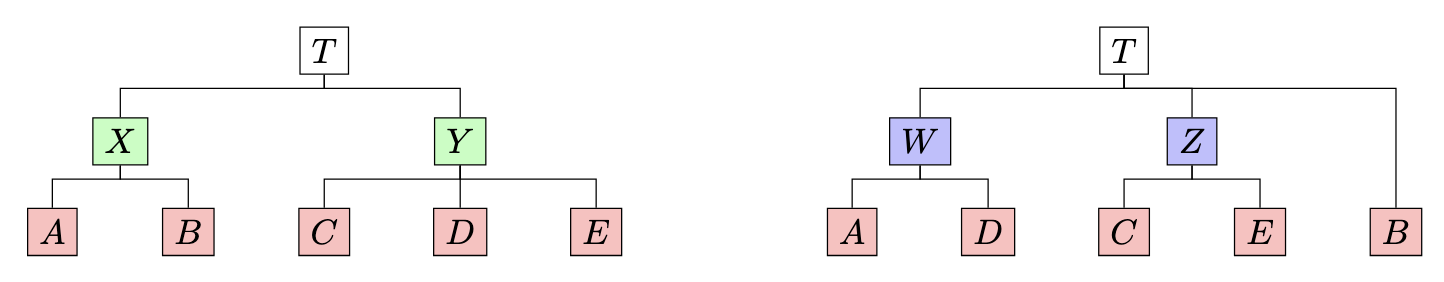
\includegraphics[width=\textwidth]{figures/comment_figure.png}
\caption{\label{fig:comment_fig}Two hierarchies that share the bottom level (in red) and the upper level (in white) series.}
\end{figure}
\vspace{-0.5cm}
\textit{We can then express the two summation matrices (see notation on page 6 ) as}
$\boldsymbol{S}_1=\left[\begin{matrix}\boldsymbol{A}\\\boldsymbol{C}_1\\\boldsymbol{I}_m\end{matrix}\right]$ \textit{and} $\boldsymbol{S}_2=\left[\begin{matrix}\boldsymbol{A}\\\boldsymbol{C}_2\\\boldsymbol{I}_m\end{matrix}\right]$ \textit{where} $\boldsymbol{C}_1=\left[\begin{matrix}
    1 & 1 & 0 & 0 & 0 \\
    0 & 0 & 1 & 1 & 1
\end{matrix}\right]$ and $\boldsymbol{C}_1=\left[\begin{matrix}
    1 & 0 & 0 & 1 & 0 \\
    0 & 0 & 1 & 0 & 1
\end{matrix}\right]$,
\textit{and we can write the} \\

\textit{grouped hierarchy as}
%\vspace{-0.2in}
\[
\boldsymbol{S}_g=\left[\begin{matrix}\boldsymbol{A} \\ \boldsymbol{C}_g \\ \boldsymbol{I}_m \end{matrix}\right] \quad\text{with}\quad \boldsymbol{C}_g =\left[\begin{matrix}
    \boldsymbol{C}_1 \\ \boldsymbol{C}_2
\end{matrix}\right] = \left[ \begin{matrix} 1 & 1 & 0 & 0 & 0 \\ 0 & 0 & 1 & 1 & 1 \\ 1 & 0 & 0 & 1 & 0 \\ 0 & 0 & 1 & 0 & 1 \end{matrix}\right].
\]
\textit{Obviously, possible duplicated series should be removed. Those we obtain a grouped hierarchy with number of middle level series $n_g$ such that $\min(n_1,n_2)\leq n_1+n_2$, where $n_1$ and $n_2$ are the number of middle level series for the ``simple'' hierarchies 1 and 2, respectively.}
\medskip

\textit{The only section where the authors consider all levels together is in the combination of reconciled forecasts in Section 6, while it would be interesting to understand if this grouped structure offers any benefit due to the increased number of middle level series.}

\medskip

\noindent \textbf{Response:} 
Thank you for the comment. We agree with the referee that it would be interesting to see if grouped structure can further improve forecast accuracy. We  have included a grouped hierarchy structure in our study, which combines the aggregation constraints of all 12 clustering-based hierarchies. Theses new results are shown in Table 3 of the revised manuscript, and also in Table \ref{tab:P2_rmsse}. We can see that the performance of the grouped hierarchy is much poorer compared to individual clustering hierarchies. We suspect this may be a consequence of having too large a hierarchy, resulting in difficulty in estimating the covariance matrix $\boldsymbol{W}$ used as an input to MinT (\citealp{pritulargaStochasticCoherencyForecast2021}). 


% \begin{table}[h!]
%     \centering
% \caption{\label{tab:P3_rmsse}Performance of cluster hierarchies and benchmark hierarchies in terms of average RMSSE across all evaluation windows on both datasets. Column-wise minimum values are displayed in bold.}
% \begin{tabular}{lrr}\toprule
%     Approach & tourism & mortality \\ \midrule
%     Base & 0.6945 & 0.7530 \\ 
%     Two-level & 0.6944 & 0.7528 \\ 
%     Natural & 0.6913 & 0.7501 \\ 
%     \color{purple}Grouped & 0.7068 & 0.8091\\
%     TS-EUC-ME & 0.6939 & 0.7528 \\ 
%     ER-EUC-ME & 0.6938 & 0.7530 \\ 
%     TSF-EUC-ME & 0.6938 & 0.7549 \\ 
%     ERF-EUC-ME & 0.6942 & 0.7532 \\ 
%     TS-EUC-HC & 0.6922 & 0.7540 \\ 
%     ER-EUC-HC & 0.6920 & 0.7507 \\ 
%     \textbf{TSF-EUC-HC} & \textbf{0.6909} & 0.7509 \\ 
%     ERF-EUC-HC & 0.6910 & 0.7501 \\ 
%     TS-DTW-ME & 0.6940 & 0.7528 \\ 
%     \textbf{TS-DTW-HC} & 0.6911 & \textbf{0.7496} \\ 
%     ER-DTW-ME & 0.6942 & 0.7531 \\ 
%     ER-DTW-HC & 0.6912 & 0.7532 \\ \bottomrule
% \end{tabular}

% \end{table}

  

\begin{table}
    \centering
    \vspace{-0.8in}
\caption{\label{tab:P2_rmsse}Performance of cluster hierarchies and benchmark hierarchies in terms of average RMSSE across all evaluation windows on both datasets. Column-wise minimum values are displayed in bold.}
\begin{tabular}{lrr}\toprule
    Approach & tourism & mortality \\ \midrule
    Base & 0.6945 & 0.7530 \\ 
    Two-level & 0.6944 & 0.7528 \\ 
    Natural & 0.6913 & 0.7501 \\ 
    Grouped & 0.7068 & 0.8091\\
    TS-EUC-ME & 0.6939 & 0.7528 \\ 
    ER-EUC-ME & 0.6938 & 0.7530 \\ 
    TSF-EUC-ME & 0.6938 & 0.7549 \\ 
    ERF-EUC-ME & 0.6942 & 0.7532 \\ 
    TS-EUC-HC & 0.6922 & 0.7540 \\ 
    ER-EUC-HC & 0.6920 & 0.7507 \\ 
    \textbf{TSF-EUC-HC} & \textbf{0.6909} & 0.7509 \\ 
    ERF-EUC-HC & 0.6910 & 0.7501 \\ 
    TS-DTW-ME & 0.6940 & 0.7528 \\ 
    \textbf{TS-DTW-HC} & 0.6911 & \textbf{0.7496} \\ 
    ER-DTW-ME & 0.6942 & 0.7531 \\ 
    ER-DTW-HC & 0.6912 & 0.7532 \\ \bottomrule
\end{tabular}

\end{table}

\textbf{Comment 12:} \textit{Page 15 rows 34--44. The example used to explain the permutation strategy employs a natural hierarchy structure. However, Figure 5 utilizes a graphical structure typical of the cluster presented in Figure 1 on the right. I suggest that the authors consider the structure in Figure 1 on the left, which is more commonly and easily identifiable as a natural hierarchy.}

\medskip

\noindent \textbf{Response:} {Thank you for your advice. Following this comment, we have revised Figure 5 of the manuscript and we are now using the structure in Figure 1 on the left for illustrative purposes. }\\



\textbf{Comment 13:} \textit{Page 15 rows 36--41. The index $l$ is not specified.}

\medskip

\noindent \textbf{Response:} {Thank you for pointing this out. We have now defined index $l$ in the text, which is the total number of hierarchies included in the forecast combination. }

\medskip

\subsection*{Minor comments \& typos}

\begin{table}[ht]
    \centering
    \resizebox{\textwidth}{!}{
    \begin{tabular}{cc|c|l|l}
    \toprule
        \thead{Page} & \thead{Row} & \thead{Errata} &\thead{Corrige} & \thead{Note} \\
        \midrule
        6 & 17--24 & $\boldsymbol{a}_t$ & $a_t$ & Remove the bold for the scalar
values \\ \midrule
7 & 34/40 & raw & original & Coherent notation as proposed in page 3 row 41 \\\midrule
7 & 50 & context time series & context of time series & \\ \midrule
26 & 7 & A review.' & \makecell{A review’, International  \\ Journal  of Forecasting, \\40(2), 430--456.} & \\\bottomrule
    \end{tabular}}
\end{table}

\medskip

\noindent \textbf{Response:} We appreciate these comments and have made corrections accordingly.  
%{\color{red} raw time series and original time series are not the same concept.} 
{Please note that the ``raw'' and ``original'' time series refer to slightly different concepts, to advoid confusion, we have revised relevant sentences on page 7 to clarify our usage of ``raw''. }



\clearpage
\newpage

\section*{Comments from Referee 2}

We appreciate your comments and we are glad that the referee found our paper interesting and well-written. Following the referee's guidance, we have made clarifications on the permutation method, and added further discussions on the performance of the natural hierarchy. Below, we present point-by-point responses to address your comments. 

\subsection*{General comments}


%\textit{An excellent, well written, interesting paper.} 


\textbf{Comment 1:} \textit{I have one main point to make. I think that you could explain a little more clearly your work in section 4. Perhaps I am being a bit slow, but I really struggled with your description of what is going on when you discuss permuting an existing `natural' hierarchy. Surely you can only do this by disregarding or dropping some or of the `bottom' intermediate levels? Otherwise the hierarchy is fully specified and I cant see how you can randomly allocate bottom level series? If I am correct in this, please try to make this clear. If I am incorrect then perhaps you still need a much better description! I think this is quite unclear, however I can see where you are going in terms of ``grouping'' v ``structure''.... you could just clarify how you get there.}

\medskip

\noindent \textbf{Response:} We appreciate these comments.
We note that the structure of the hierarchy remains unchanged while all bottom level series are retained (they are simply permuted). In practice, \textit{all} middle level time series are dropped. When randomly shuffling the bottom level series, some middle level series of the natural hierarchy could be retained by chance, although this is highly unlikely. We understand where the confusion could arise, therefore we have revise the description of the permuted hierarchy in Section 4. In particular, we now work through the example in Figure 5 in detail, making it clear how the middle level series change as a result of the permutation. \\



%that and we thank you for bringing this to our attention. Add comment in text making it clear that the forecasts of small population states can only borrow strength if they have neighbours. 




\textbf{Comment 2:} \textit{In terms of your broad conclusion it is interesting that the natural hierarchy performs more or less as well as the statistically generated ones. Obviously the natural hierarchy contains `prior' information\ldots which your statistical methods ignore. This may be a good reason why the natural hierarchy does well?}

\medskip

\noindent \textbf{Response:} Thank you for your comment. We fully agree with you that the natural hierarchy contains important prior information of the dataset, which may not have been taken into account in the clustering-based hierarchy construction. For example, tourist data from the same state are likely to be affected by common shocks and dynamics. This in turn, can potentially explain the competitive performance of the natural hierarchy compared to the other structures. In the revised manuscript, we have added this discussion in Sections 3.3. 


\clearpage
\newpage

\bibliography{references.bib}
\end{document}